% !TEX root = ../../../main.tex
% 来源：高中物理甲种本·第一册（力学）
% 章节：力 / 力的合成的计算
% 原始文件：1.tex，行 1209-1220
% 类型：tikz
% ---
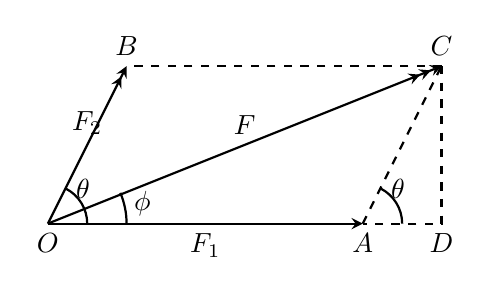
\begin{tikzpicture}[>=stealth,  thick]
\draw [->](0,0)node[below] {$O$}--node[below] {$F_1$} (4,0)node[below] {$A$} ;
\draw [->>](0,0)--node[above] {$F_2$}(1,2) node[above] {$B$};
\draw [dashed](5,2)--(1,2);
\draw [dashed](4,0)--(5,2)node[above] {$C$};
\draw [->>>](0,0)--node[above] {$F$}(5,2) ;
\draw [dashed](5,2)--(5,0) node[below] {$D$}--(4,0);
\draw (.5,0) arc (0:63:.5) node[right] {$\theta$};
\draw (1,0) arc (0:23:1);
\draw (4.5,0) arc (0:63:.5) node[right] {$\theta$};
\node at (1.2,.25) {$\phi$};
\end{tikzpicture}
